% Based on: https://github.com/martinhelso/OsloMet


\documentclass[UKenglish, aspectratio = 169]{beamer}
\usepackage[utf8]{inputenc}

\usetheme{OsloMet}
\usepackage{style}

\usepackage{tabularx, booktabs, makecell, adjustbox}

\usepackage{hyperref}
\usepackage{framed}

\definecolor{shadecolor}{gray}{0.9}

\usepackage{tikz, pgfplots}
\usetikzlibrary{shapes.geometric, arrows, positioning}

% % Tikz Definitions % % % % % % % % % % % % % % % % % % % %

\tikzstyle{normalnode} = [rectangle, rounded corners, minimum width=2cm, minimum height=1cm,text centered, text width=2.5cm, draw=black]
\tikzstyle{arrow} = [thick,>=stealth,->]



% % Tikz Definitions % % % % % % % % % % % % % % % % % % % %


\newcommand{\etal}{\textit{et al.}}
\newcommand{\TODO}[1]{{\Large \color{red} TODO: #1}}

\author[Torras \textit{\etal}]
{Pau Torras -- \texttt{ptorras@cvc.uab.cat}
\texorpdfstring{\\}{}
Sanket Biswas
\texorpdfstring{\\}{}
Alicia Fornés
}

\cvcaffiliation{
    Computer Vision Center, Universitat Autònoma de Barcelona
}


\title{A Unified Representation Framework for the Evaluation of Optical Music Recognition Systems}
\subtitle{}


\begin{document}

% Use
%
%     \begin{frame}[allowframebreaks]
%
% if the TOC does not fit one frame.
\begin{frame}{Table of contents}
    \tableofcontents
\end{frame}


% % % % % % % % % % % % % % % % % % % % % % % % % % % % % % % % % % % % % % % % 
% Motivation
% % % % % % % % % % % % % % % % % % % % % % % % % % % % % % % % % % % % % % % %

\section{Motivation}
\SectionPage

\hidelogo
\begin{frame}[c]{Optical Music Recognition (OMR)}
	\begin{figure}
		\includegraphics[width=0.9\textwidth]{images/omr.pdf}
	\end{figure}
\end{frame}
\showlogo

\begin{frame}[c]{The Requirements of OMR}
	We identify a few key requirements that have not yet been addressed in OMR
	
	\begin{itemize}
	 	\item \textbf{A standardised output:} Most OMR systems assume different
	 	collections of objects and semantics as output.
	 	\item \textbf{Evaluation Metrics:} Measuring the quality of OMR systems 
	 	fairly and equitably is currently not possible.
	\end{itemize}
	\textbf{Both of these issues are intertwined:} Unless defined on the 
	same representation, fair evaluation metrics are not possible
\end{frame}

% % % % % % % % % % % % % % % % % % % % 

\begin{frame}[c]{An important side note}
	The focus of this work is on \textbf{fully structured encodings} of music, as 
	defined in \cite{calvo-zaragoza_understanding_2021}.
	
	\begin{center}
\begin{tikzpicture}[align=center, node distance=3.5cm]
	\node (meta) [normalnode, fill=cvcred!10] {Metadata Extraction};
	\node (search) [normalnode, right of=meta, fill=cvcred!25] {Search};
	\node (repl) [normalnode, right of=search, fill=cvcred!40] {Replayability};
	\node (struct) [normalnode, right of=repl, fill=cvcred!55] {Structured Encoding};
	
	\draw [arrow] (meta) -- (search);
	\draw [arrow] (search) -- (repl);
	\draw [arrow] (repl) -- (struct);
	
	\draw[->,ultra thick] (-1,-1)--(9,-1) node[right]{Comprehension};
\end{tikzpicture}
\end{center}
	
	We only consider the application on \textbf{Common Western Music Notation}.
\end{frame}

% % % % % % % % % % % % % % % % % % % % 

\hidelogo
\begin{frame}[c]{A Taxonomy of Music Representations}
	\only<1>{
		\begin{figure}
			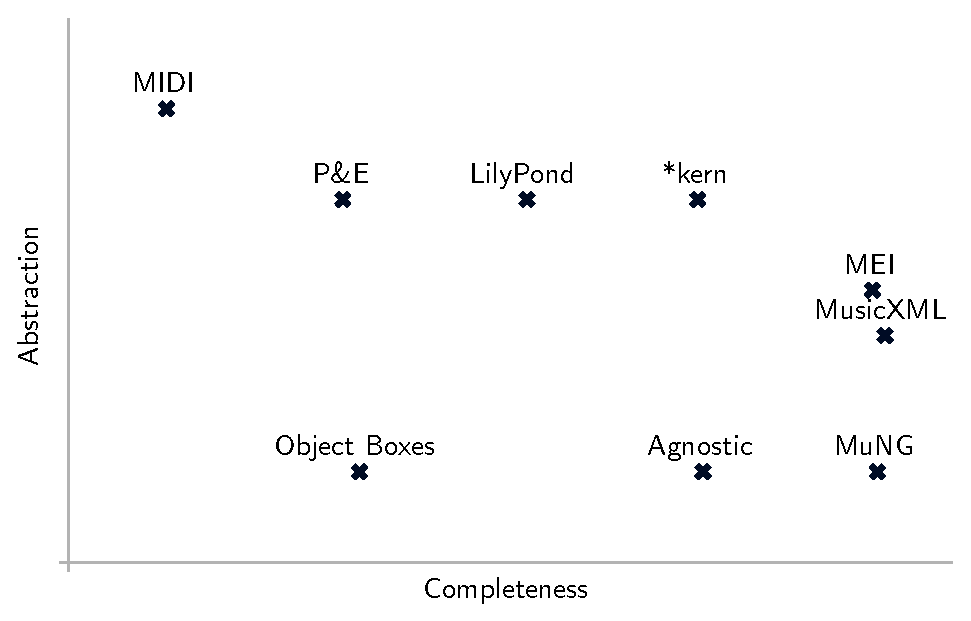
\includegraphics[width=.8\textwidth]{diagrams/fig_formats.eps}
		\end{figure}
	}
	\only<2>{
		\begin{figure}
			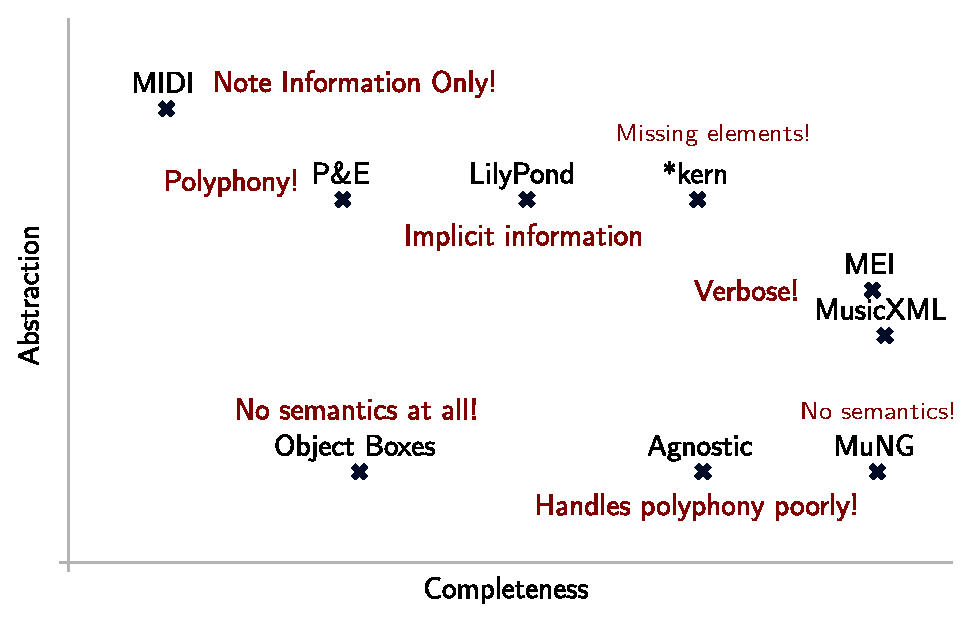
\includegraphics[width=.8\textwidth]{diagrams/fig_formats_downsides.eps}
		\end{figure}
	}
\end{frame}
\showlogo

% % % % % % % % % % % % % % % % % % % % 

\begin{frame}[c]{A Taxonomy of Music Representations}
	Outside of OMR, complex scores are usually engraved using
	\begin{itemize}
		\item \textbf{MusicXML:} Particularly in large repository sites and most 
		musicological applications
		\item \textbf{MEI:} It is lately getting traction in mainstream applications as
		well as its original archive-focused domain.
	\end{itemize}
	\only<2>{
		\begin{alertblock}{Nevertheless...}
			It is not trivial to work with these formats for OMR. It is possible, but 
			some simplifying assumptions must be made 
			\cite{mayerPracticalEndtoEndOptical2024}.
		\end{alertblock}
	}
\end{frame}

% % % % % % % % % % % % % % % % % % % % 

\begin{frame}[c]{OMR Datasets}
	\resizebox{\columnwidth}{!}{%
\begin{tabular}{@{}lllll@{}}
\toprule
Publication                         & Dataset Name       & Score Type & Document Type      & Annotation Type \\ \midrule
\cite{hajic_muscima_2017}           & MUSCIMA++          & CWMN       & Modern Handwritten & MuNG            \\
\cite{tuggener_deepscores_2018, tuggener_deepscoresv2_2020} & DeepScores    & CWMN     & Typeset                & Bounding Boxes \\
\cite{tuggener_real_2023}           & RealScores         & CWMN       & Scanned Typeset    & Bounding Boxes  \\
\cite{shatri_doremi_2021}           & DoReMi             & CWMN       & Typeset            & Multiple        \\
\cite{parada-cabaleiro_seils_2017}                          & SEILS         & Mensural & Scanned Typeset        & Agnostic + MEI \\
\cite{baro_handwritten_2020}        & Baró Synthetic     & CWMN       & Typeset            & Agnostic        \\
\cite{baro_handwritten_2020}                                & Pau Llinás    & CWMN     & Historical Handwritten & Agnostic       \\
\cite{calvo-zaragoza_end--end_2018} & PRIMuS             & CWMN       & Typeset            & Agnostic + MEI  \\
\cite{calvo-zaragoza_camera-primus_2018}                    & Camera PRIMuS & CWMN     & Typeset (Scan-like)    & Agnostic + MEI \\
\cite{rios-vila_end--end_2023}      & GrandStaff         & CWMN       & Typeset            & *kern           \\
\cite{stringquartet_corpus}         & OpenScore Quartets & CWMN       & Typeset            & MuseScore       \\
\cite{GothamJonas2022}              & OpenScore Lieder   & CWMN       & Typeset            & MuseScore       \\ \bottomrule
\end{tabular}%
}
\end{frame}

% % % % % % % % % % % % % % % % % % % % 

\begin{frame}[c]{So, what should we do?}
	\begin{itemize}
		\item We have to try and find a way to connect all of these isolated datasets
		and formats and find a way of representing them using the same language.
		\begin{itemize}
			\item The main goal is \textbf{evaluation}, but having such a tool could 
			improve researchers' QOL by standardising an output for all of OMR, 
			\textbf{making it possible to share tools and efforst more easily}.
		\end{itemize}
		
		\item None of the existing formats are completely suitable for a majority 
		of use cases within OMR.

		\item Therefore, \textbf{we built one with these in mind}.
	\end{itemize}		
\end{frame}

% % % % % % % % % % % % % % % % % % % % 

\hidelogo
\begin{frame}[c]{Why design a new format?}
	\begin{figure}
		\includegraphics[width=.8\textwidth]{images/standards_2x.png}
		
	\end{figure}
	\href{https://xkcd.com/927/}{``Standards''} by XKCD, \href{https://creativecommons.org/licenses/by-nc/2.5/}{CC-BY-NC 2.5} 
	
\end{frame}
\showlogo

% % % % % % % % % % % % % % % % % % % % 

\begin{frame}[c]{Why design a new format?}
	\only<1->{
		\begin{alertblock}{Reason \#1}
			Fair evaluation must be possible regardless of the original
			annotation format of the material.
		\end{alertblock}
	}

	
	\only<1>{
		The point of agreement of all sources is the presentation of the score.
		\begin{center}
			``Engraving that can be processed''
		\end{center}
		
		\begin{example}
			The SVG output of the Verovio engraving software.
		\end{example}
	}
	
	\only<2>{
	\begin{itemize}
		\item This has the effect of \textbf{standardising how to deal with each 
		format's assumptions}.
		\item ... but a notation like this does not really exist yet!
	\end{itemize}
	}

\end{frame}


% % % % % % % % % % % % % % % % % % % % 

\begin{frame}[c]{Why design a new format?}
	\begin{alertblock}{Reason \#2}
		There must only be \textbf{one} way to represent each score.
	\end{alertblock}
	
	Most formats have semantic constructs that allow equivalent representations of a 
	score, which can make evaluation metrics meaningless in some contexts.
	
	\begin{figure}
		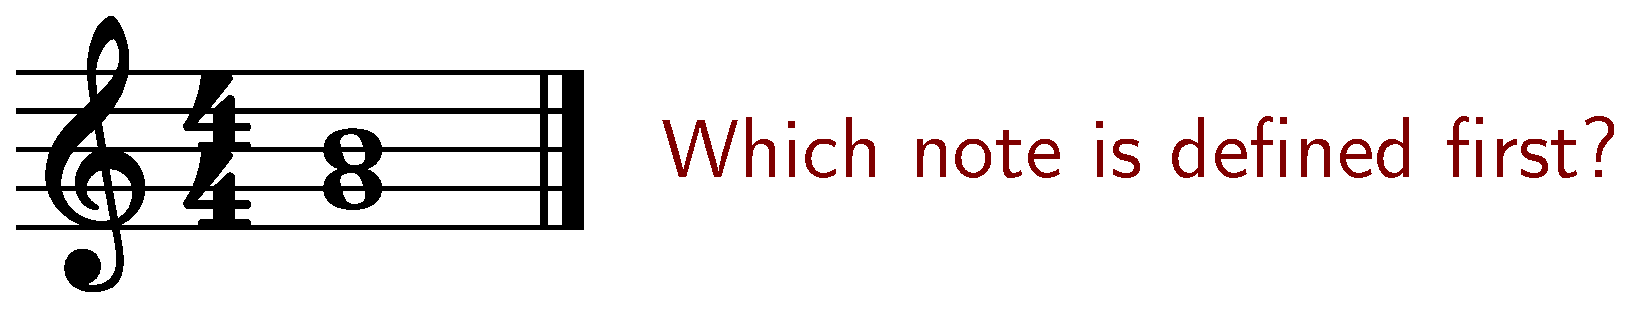
\includegraphics[width=.7\textwidth]{diagrams/fig_ordering}
	\end{figure}

\end{frame}

% % % % % % % % % % % % % % % % % % % % 

\begin{frame}[c]{Why design a new format?}
	\only<1->{
		\begin{alertblock}{Reason \#3}
			The representation must be \textbf{faithful} and \textbf{exhaustive}.
		\end{alertblock}
	}
	
	\only<1>{
		\begin{figure}
			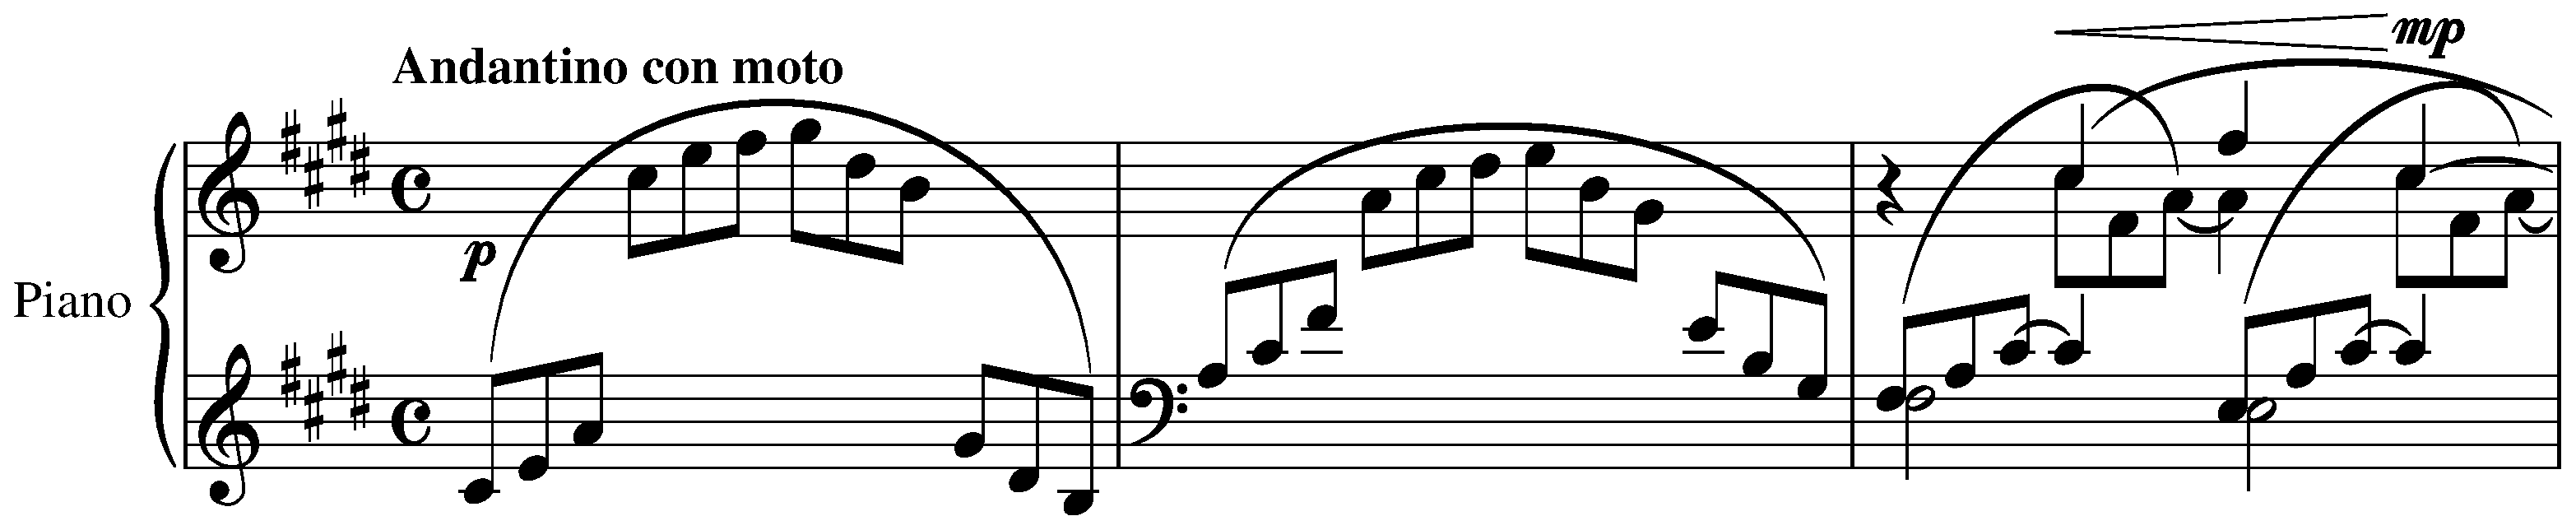
\includegraphics[width=.7\textwidth]{images/arabesques_verovio.eps}
			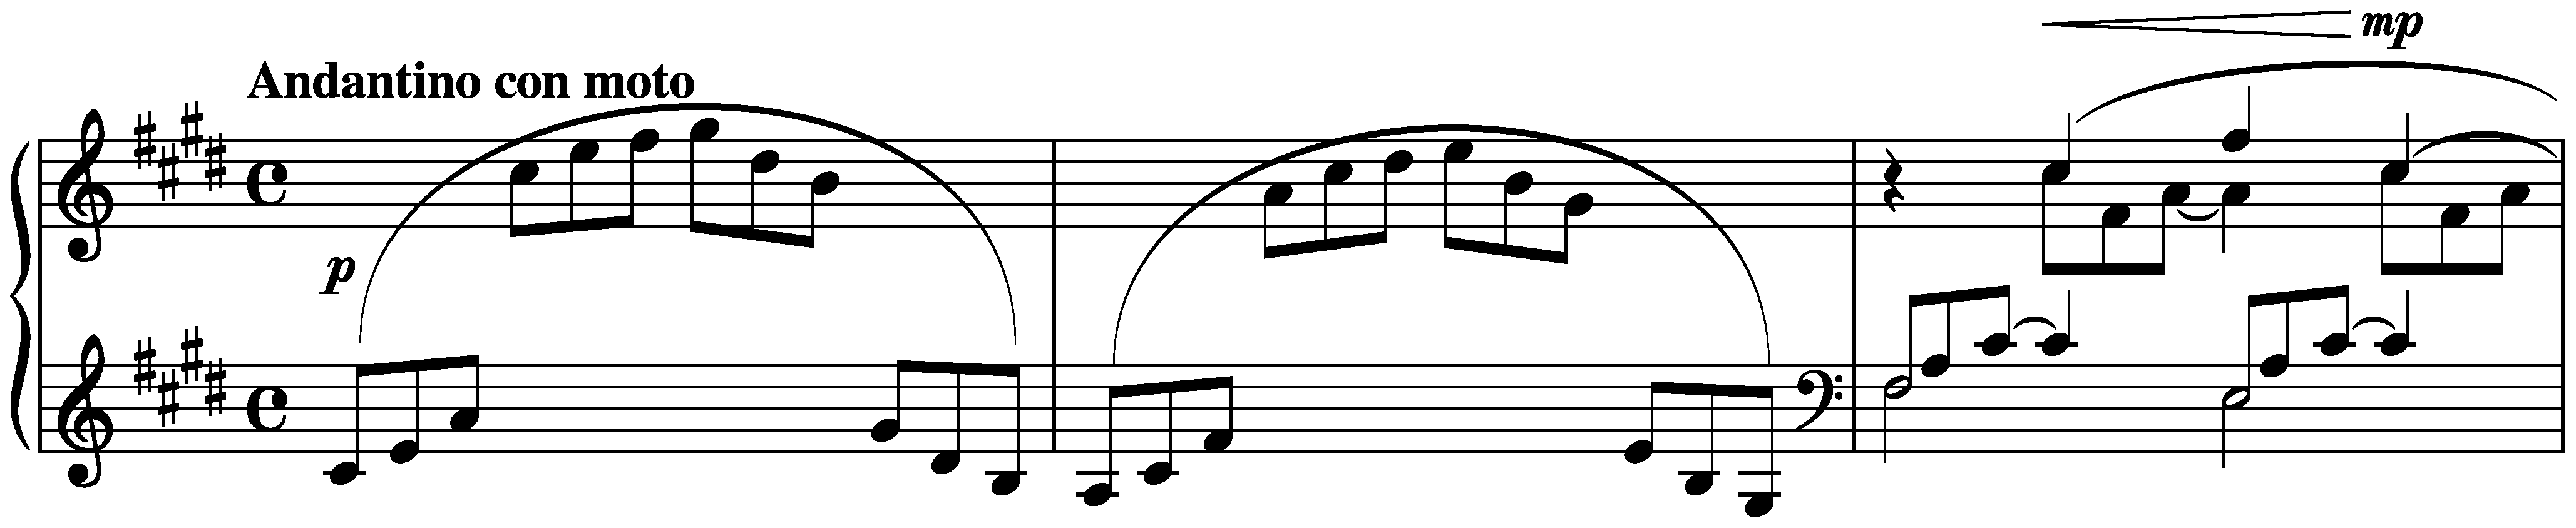
\includegraphics[width=.7\textwidth]{images/arabesques_musescore.eps}
		\end{figure}
	}
	\only<2>{
		\begin{itemize}
			\item These issues can sometimes be sidestepped by using optional features 
			or modifying file structures \textbf{$\rightarrow$ Need to be standardised 
			anyway}
		\end{itemize}
	}

\end{frame}

% % % % % % % % % % % % % % % % % % % % 

\begin{frame}[c]{Why design a new format?}
	\begin{alertblock}{Reason \#4}
		Semantics and presentation must be separate.
	\end{alertblock}
	
	From \cite{calvo-zaragoza_understanding_2021}
	
	\begin{quote}
		In particular, there is no known meaningful edit distance between two 
		scores 
		[...] However, this does not necessarily provide a good measure of quality, 
		because it is unclear how to weight the costs of different edit operations, 
		e.g., getting a note duration wrong vs. missing an articulation mark.
	\end{quote}
\end{frame}

% % % % % % % % % % % % % % % % % % % % 

\begin{frame}[c]{Why design a new format?}
	\begin{alertblock}{Reason \#5}
		We need to communicate with the rest of the ecosystem.
	\end{alertblock}
	
	We need tools that facilitate using external sources and exporting our results.
\end{frame}


% % % % % % % % % % % % % % % % % % % % 

\begin{frame}[c]{Wrapping up}
	We decided to prototype a representation that encapsulates all of these requirements. 
	We call it Music Tree Notation, or \textbf{MTN}.
\end{frame}

% % % % % % % % % % % % % % % % % % % % % % % % % % % % % % % % % % % % % % % % 
% Design
% % % % % % % % % % % % % % % % % % % % % % % % % % % % % % % % % % % % % % % %

\section{Design}
\SectionPage

% % % % % % % % % % % % % % % % % % % % 

\begin{frame}[c]{An Overview}
	\only<1>{
	\begin{figure}
		\includegraphics[height=.8\textheight, page=1]{ppt_diagrams/schematic_full.pdf}
	\end{figure}
	}
	\only<2>{
	\begin{figure}
		\includegraphics[height=.8\textheight, page=2]{ppt_diagrams/schematic_full.pdf}
	\end{figure}
	}
	\only<3>{
	\begin{figure}
		\includegraphics[height=.8\textheight, page=3]{ppt_diagrams/schematic_full.pdf}
	\end{figure}
	}
	\only<4>{
	\begin{figure}
		\includegraphics[height=.8\textheight, page=4]{ppt_diagrams/schematic_full.pdf}
	\end{figure}
	}
	\only<5>{
	\begin{figure}
		\includegraphics[height=.8\textheight, page=5]{ppt_diagrams/schematic_full.pdf}
	\end{figure}
	}
	
\end{frame}

% % % % % % % % % % % % % % % % % % % % 

\hidelogo
\begin{frame}[c]{The format}
	\begin{figure}
		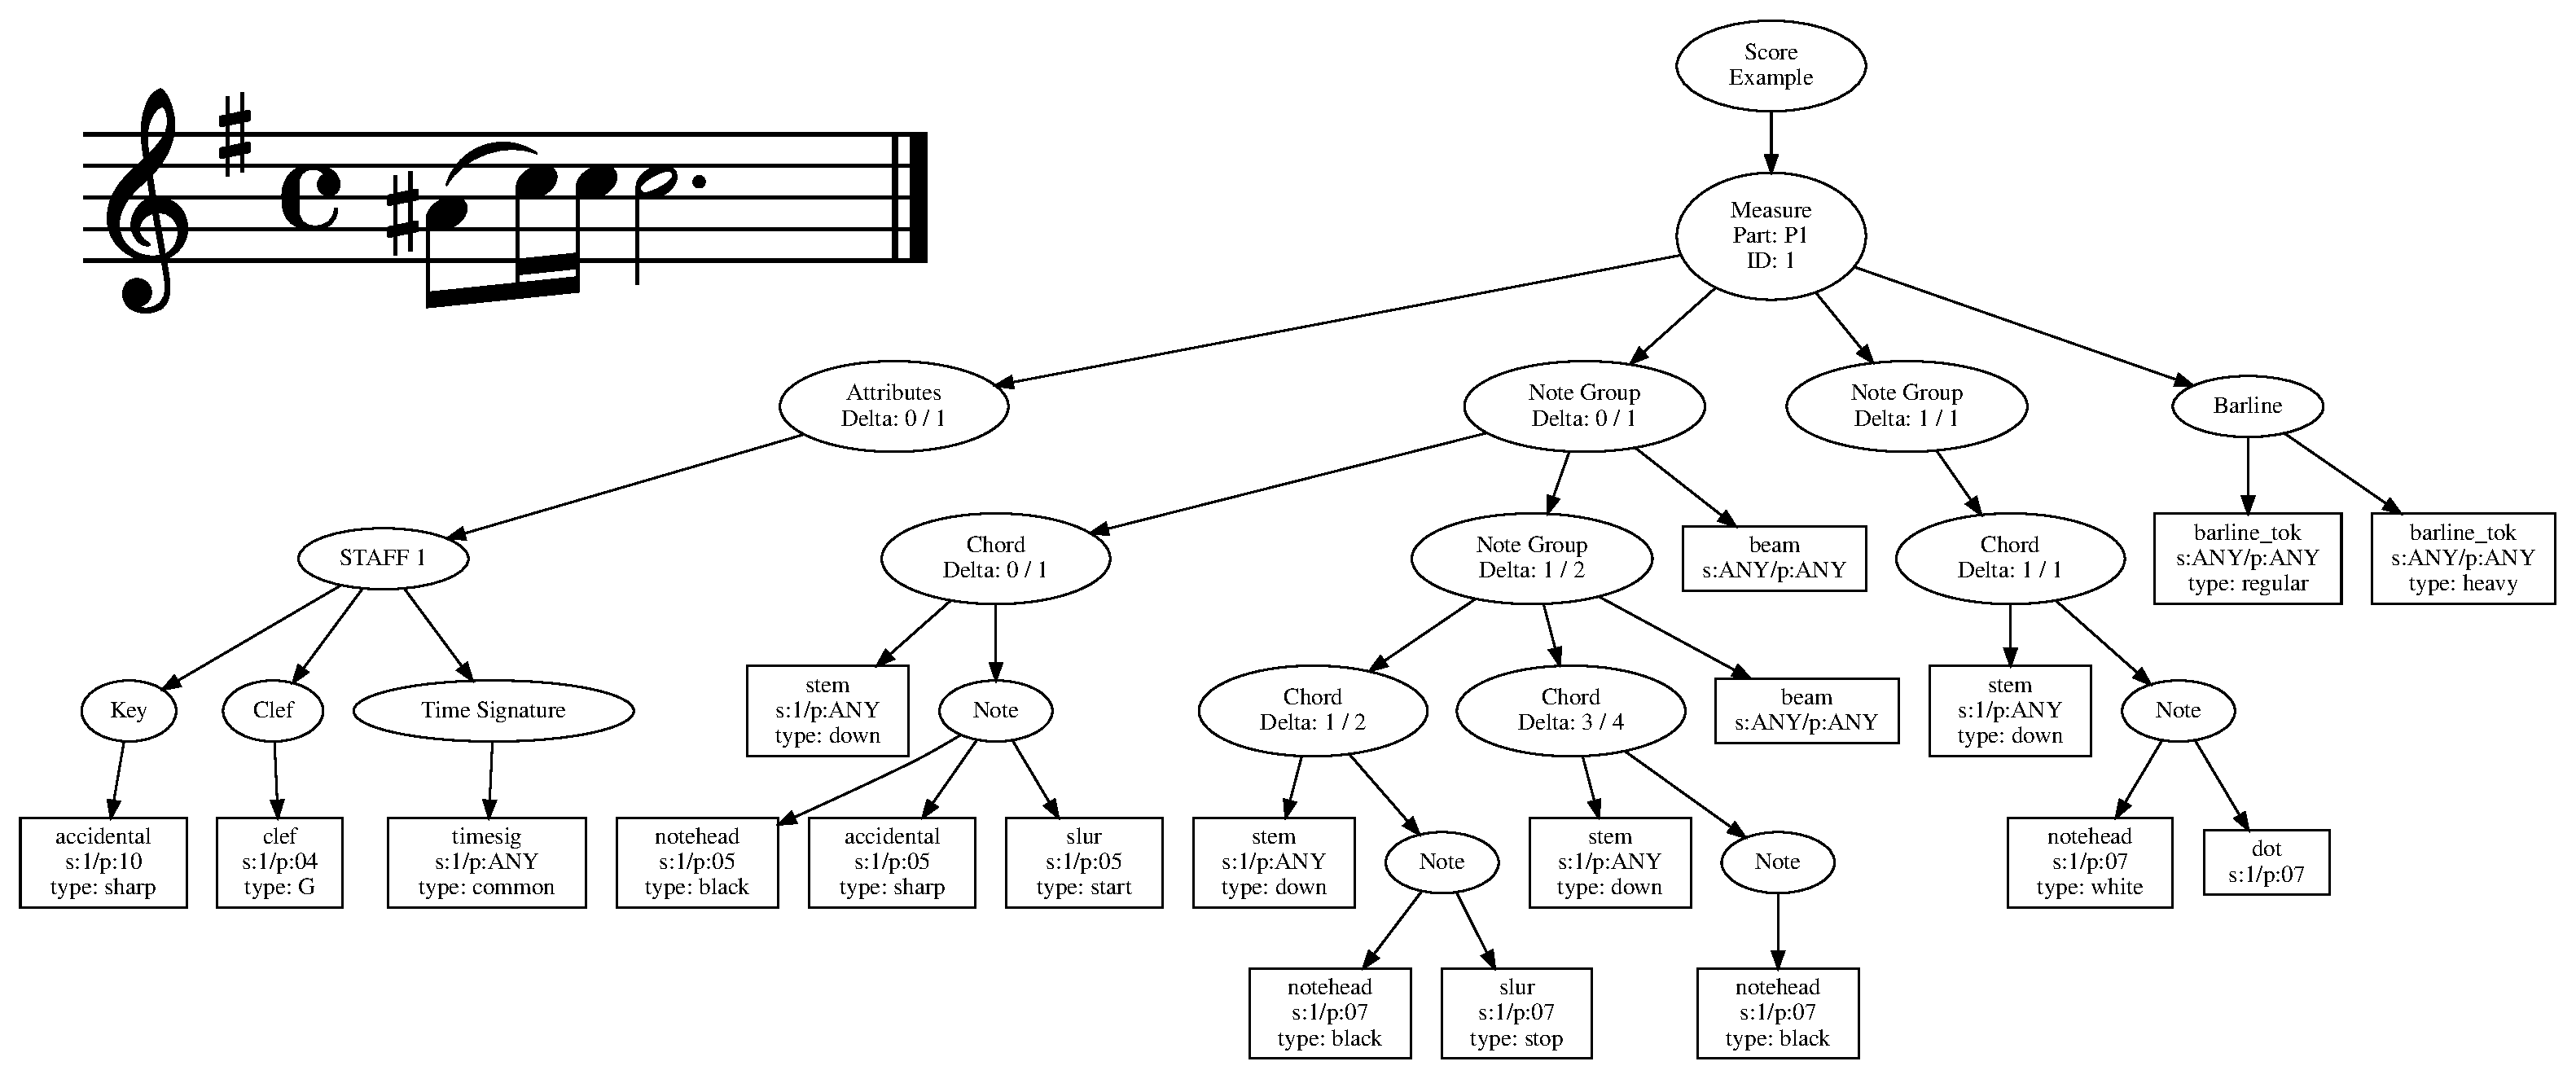
\includegraphics[height=.7\textheight]{diagrams/new_figure_demo.eps}
	\end{figure}
\end{frame}
\showlogo

% % % % % % % % % % % % % % % % % % % %

\begin{frame}[c]{Key aspects of the format}
	\begin{itemize}
		\item<1-> \textbf{Tree data structure:} Intuitively follows music rules, many 
		algorithms available, mimicks abstract parse tree.
		\item<2-> \textbf{Time information:} Required, added mostly for sync. 
		\textbf{Columns}
		\item<2-> \textbf{Placement Information:} Objects that have placement rules 
		incorporate staff and line.
		\only<2>{
			\begin{figure}
				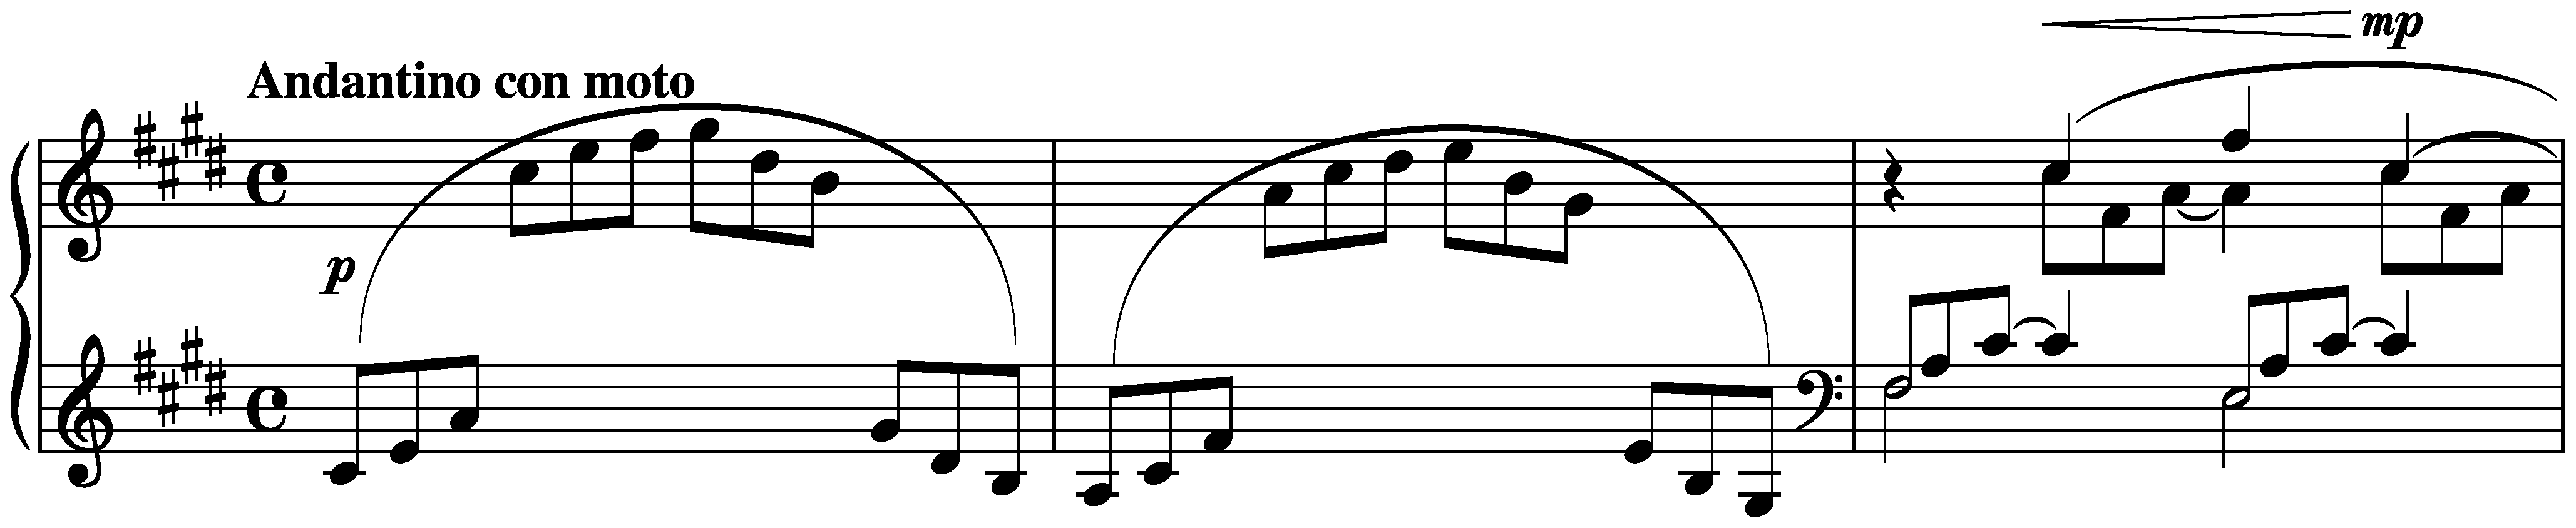
\includegraphics[width=.7\textwidth]{images/arabesques_musescore.eps}
			\end{figure}
		}
		\item<3-> \textbf{Measures are self-contained:} Semantics are parsed \textit{a 
		posteriori}.
		\item<4-> \textbf{Exchange formats:} We packaged it through XML.
	\end{itemize}
\end{frame}

% % % % % % % % % % % % % % % % % % % %


\begin{frame}[c]{Metrics}
	\begin{itemize}
		\item<1-> \textbf{Tier 0:} Methodology-specific metrics
		\only<1> {
			\begin{itemize}
				\item \textit{Whatever is defined for an existing approach}
			\end{itemize}					
		}
		\item<2-> \textbf{Tier 1:} Primitive detection
		\only<2> {
			\begin{equation*}
				\text{precision} = \frac{\|P \cap G\|}{\|P\|}
			\end{equation*}		
		    \begin{equation*}
		        recall = \frac{\|P \cap G\|}{\|G\|}
		    \end{equation*}						
		}
		\item<3-> \textbf{Tier 2:} Structure reconstruction
		\only<3>{
		\begin{equation*}
		    TER = \frac{S + D + I}{\|G\|}
		\end{equation*}
		}
		\item<4-> \textbf{Tier 3:} Semantic reconstruction
		\only<4>{
			\begin{equation*}
    			MNR = \frac{\| \left\{ n_g \in G : (n_p, n_g) \notin M, \forall n_p \in P \right\} \|}{\| G \|}.
			\end{equation*}
			\begin{equation*}
    			\text{Pitch Precision} = \frac{\| \left\{ (n_p, n_g) \in M : p_{n_p} = p_{n_g} \right\} \|}{\| M \|}.
			\end{equation*}
			\begin{equation*}
    			\text{Avg. Pitch Shift} = \frac{1}{\| M \|} \sum_{\forall (n_p, n_g) \in M} p_{n_p} - p_{n_g}.
			\end{equation*}
		}
	\end{itemize}
\end{frame}

% % % % % % % % % % % % % % % % % % % % % % % % % % % % % % % % % % % % % % % % 
% A proof-of-concept
% % % % % % % % % % % % % % % % % % % % % % % % % % % % % % % % % % % % % % % %

\section{Proof-of-concept}
\SectionPage


\begin{frame}[c]{A simple baseline: Dataset}
	\begin{itemize}
		\item Lieder Corpus, String Quartet Corpus \cite{gotham_scores_2018} and 
		miscellaneous OpenScore project CC0 transcriptions, totalling 894 MusicXML 
		files.
		\item Creation of a dataset at measure and page-level and testing it on an 
		OMR system.
		\item \textbf{88 Classes}.
	\end{itemize}
\end{frame}

% % % % % % % % % % % % % % % % % % % %


\begin{frame}[c]{A simple baseline: Dataset}
	\begin{figure}
		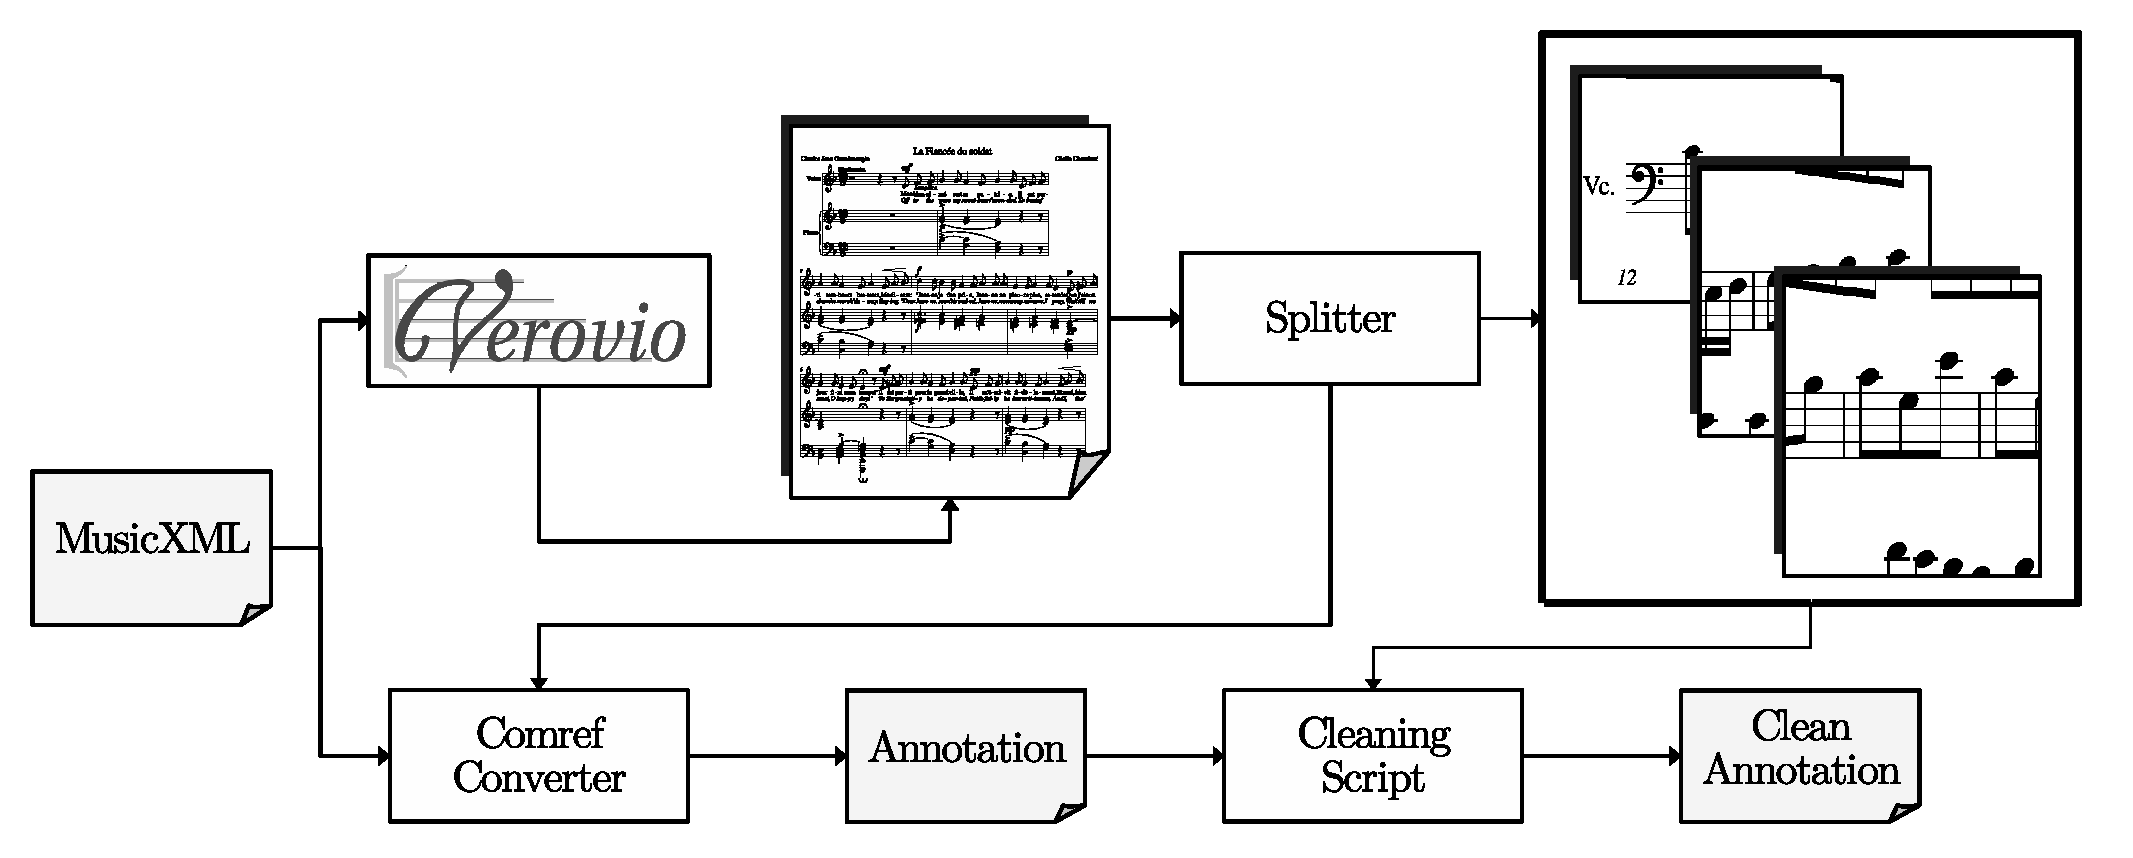
\includegraphics[width=.9\textwidth]{diagrams/dataset_generation.eps}
	\end{figure}
\end{frame}

% % % % % % % % % % % % % % % % % % % %

\begin{frame}[c]{A simple baseline: Dataset}
	\begin{figure}
		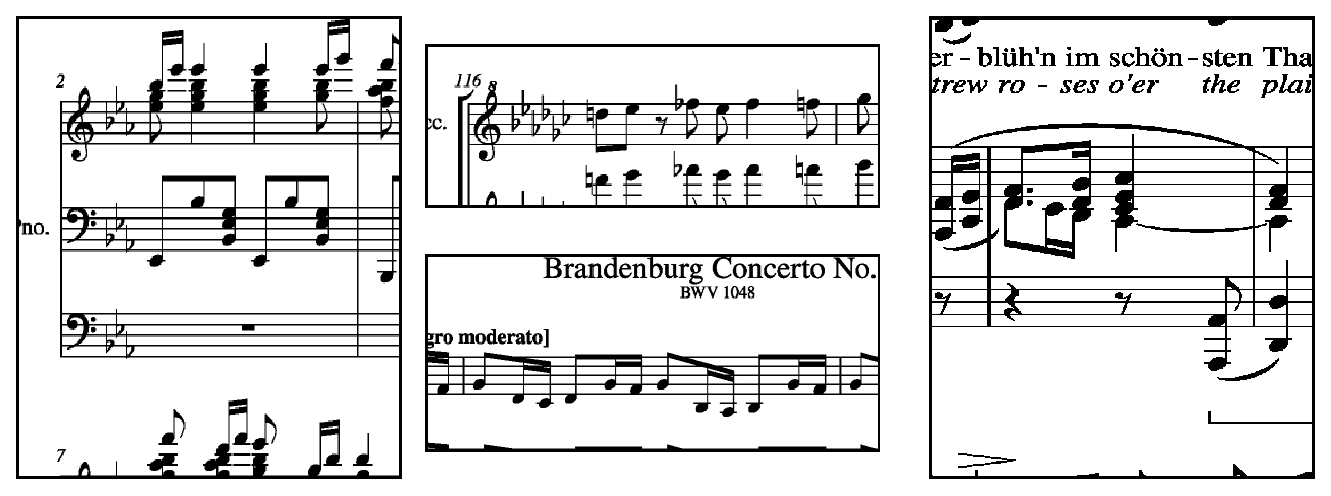
\includegraphics[width=.9\textwidth]{images/dataset_examples.eps}
	\end{figure}
\end{frame}


% % % % % % % % % % % % % % % % % % % %

\hidelogo
\begin{frame}[c]{A simple baseline: First approach}
	\begin{figure}
		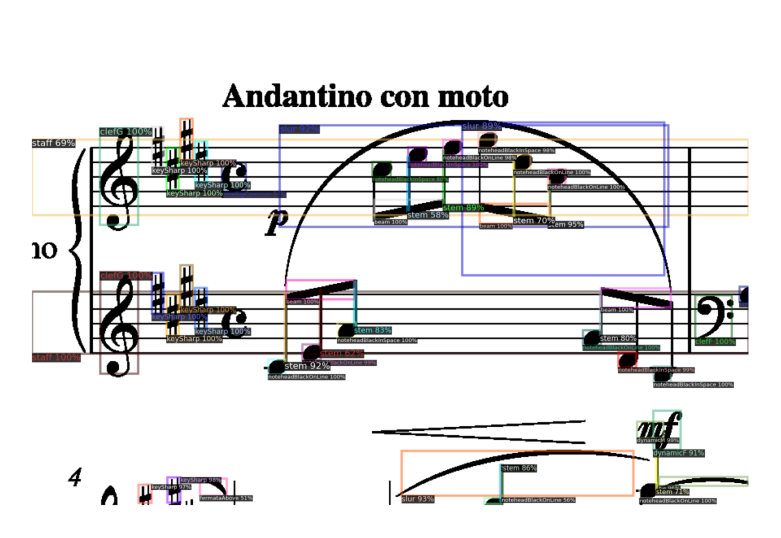
\includegraphics[width=.8\textwidth]{images/predictions.eps}
	\end{figure}
\end{frame}
\showlogo

% % % % % % % % % % % % % % % % % % % %

\begin{frame}[c]{A simple baseline: Audiveris}
	\begin{itemize}
		\item Off-the-shelf Open Source OMR system for typeset scores - Page Level.
		\item 45822 predicted measures from the 52884 present on the test set.
		\item Out of these, 40622 measures from both sets could be matched together, corresponding to a coverage of 76.9\%.
		\item \textbf{Simple Matching algorithm based on page order.}
	\end{itemize}
\end{frame}

% % % % % % % % % % % % % % % % % % % %

\hidelogo
\begin{frame}[c]{A simple baseline: Audiveris}
	\begin{figure}
		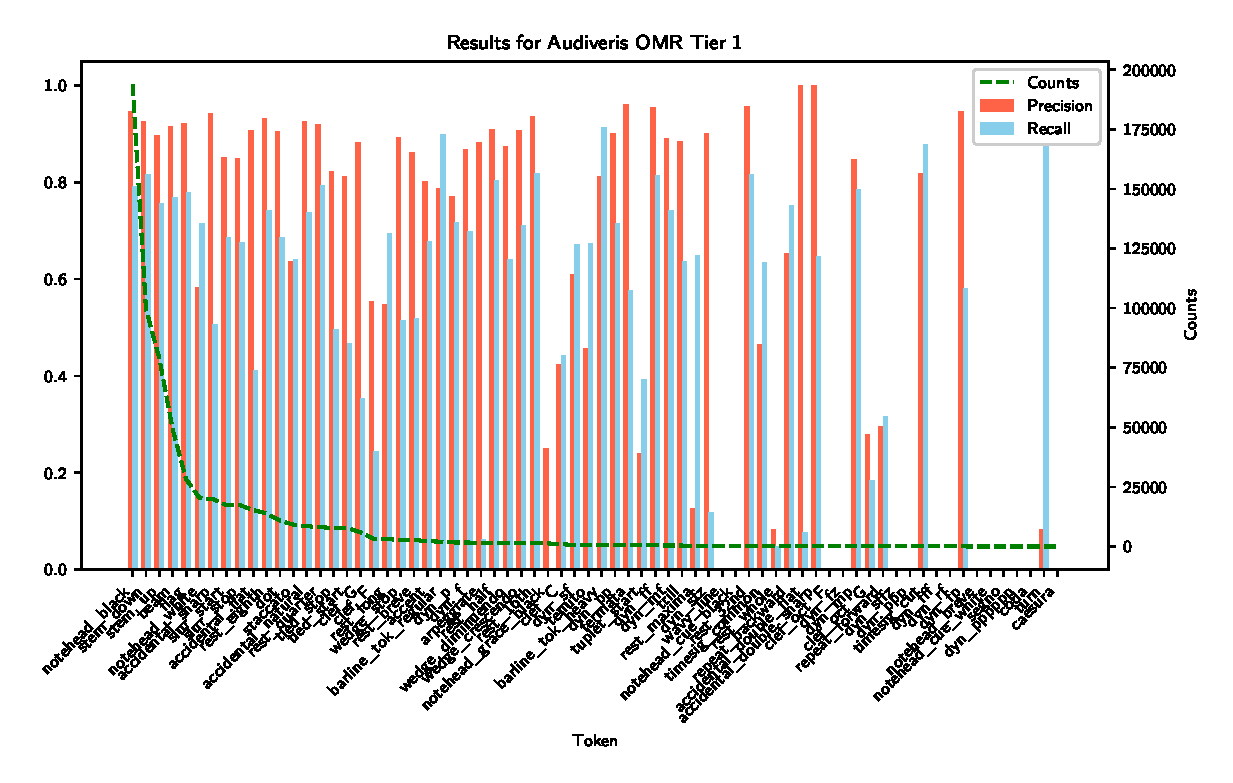
\includegraphics[width=.88\textwidth]{images/tier1.eps}
	\end{figure}
\end{frame}
\showlogo

% % % % % % % % % % % % % % % % % % % %

\begin{frame}[c]{A simple baseline: Audiveris}
	\resizebox{\columnwidth}{!}{%
\begin{tabular}{@{}ccccccccc@{}}
\toprule
TER   & Time Shift     & Pitch Shift     & Staff Shift    & Time Prec.    & Pitch Prec.    & Staff Prec.    & FPR   & MNR   \\ \midrule
0.372 & -0.096 & -0.091 & 0.022 & 0.802 & 0.749 & 0.963 & 0.097 & 0.216 \\ \bottomrule
\end{tabular}
}
\end{frame}


% % % % % % % % % % % % % % % % % % % % % % % % % % % % % % % % % % % % % % % % 
% Conclusions
% % % % % % % % % % % % % % % % % % % % % % % % % % % % % % % % % % % % % % % %

\section{Conclusions}
\SectionPage

\begin{frame}[c]{Conclusions \& Future Work}
	\begin{itemize}
		\item<1-> We have proposed a notation format for OMR.
		\item<1-> We have proposed an accompanying set of metrics.
		\item<1-> We have tested this approach with an off-the-shelf OMR system.

	\end{itemize}
	
	\only<2->{As future work:
		\begin{itemize}
			\item Support more formats
			\item Accomodate widespread adoption
			\item Construct a dataset with object bounding boxes as well.
			\item Adjust abstractions to simplify processing.
		\end{itemize}
		}
\end{frame}

\begin{frame}{Repository}
	\begin{figure}
		
\includegraphics[height=.9\textheight]{images/qr_code.eps}
	\end{figure}
\end{frame}

\begin{frame}[c]{Acknowledgements}

\textbf{We gratefully thank the participation of Carles Badal and Jan Hajič Jr. in discussions that led to improvements on this work.}

\vspace{1cm}

\begin{small}	
This work has been partially supported by the Spanish projects PID2021-126808OB-I00 (GRAIL) and CNS2022-135947 (DOLORES). Pau Torras is funded by the Spanish FPU Grant FPU22/00207 and developed part of this work while funded by the AGAUR Joan Oró FI grant 2023 FI-1-00324. The authors acknowledge the support of the Generalitat de Catalunya CERCA Program to CVC’s general activities.
\end{small}


\end{frame}

\begin{frame}[allowframebreaks]{References}
	\bibliographystyle{apalike}
	\bibliography{bibliography}
\end{frame}

\end{document}

% Pau Torras is a Second-Year Ph. D. Student at the Computer Vision Center in Barcelona. His main interests lie at the confluence of Computer Science and the Humanities. The main topic of his thesis is Optical Music Recognition applied to historical handwritten scores, but he has also worked in Ciphered Document Recognition and NLP.
